\documentclass[lettersize,journal]{IEEEtran}

\usepackage{amsmath,amsfonts,amssymb}
\usepackage{algorithmic}
\usepackage{algorithm}
\usepackage{array}
\usepackage{booktabs}
\usepackage{graphicx}
\usepackage{cite}
\usepackage{url}
\usepackage{hyperref}
\usepackage{microtype}
\usepackage{xcolor}

% Graphicspath to locate figures
\graphicspath{{./}{./docs/images/}}

\hypersetup{
    colorlinks=true,
    linkcolor=black,
    citecolor=blue!70!black,
    urlcolor=blue!70!black
}

\begin{document}

\title{Q-LATTE: QoS-Aware and Workload-Adaptive Local-Cloud Hybrid Storage for Multi-Tenant Cloud Instances}

\author{Yizreel~Schwartz~Sipahutar%
\thanks{Yizreel Schwartz Sipahutar is with the Department of Informatics, Institut Teknologi Del, Laguboti, North Sumatra, Indonesia (e-mail: yizreelschwartz180304@gmail.com). Source code and reproduction artifacts: \url{https://github.com/codenameyizzz/Reproducing-Cloud-Local-Storage-Evolution-LATTE-Hybrid-Tiering-USENIX-FAST-26}.}%
}

\markboth{IEEE Computer Architecture Letters,~Vol.~XX, No.~X,~2026}%
{Sipahutar: Q-LATTE: QoS-Aware Local-Cloud Hybrid Storage}

\maketitle

\begin{abstract}
Cloud local storage has transitioned through three generations: software polling (ESPRESSO), ASIC hardware offloading (DOPPIO), and ASIC/SoC co-design (RISTRETTO). The state-of-the-art hybrid architecture (LATTE, USENIX FAST '26) bridges physical drive limitations by pairing local flash with Elastic Block Store (EBS) via an open-source Cloud Storage Acceleration Layer (CSAL) and a Linear-SVM dispatcher. However, in shared multi-tenant cloud deployments, simultaneous I/O bursts induce severe Quality-of-Service (QoS) degradation, causing up to $3.8\times$ tail-latency spikes at P99.9. Moreover, existing single-tenant dispatchers fail to detect workload phase shifts. We propose \textbf{Q-LATTE}, an open-source, QoS-aware hybrid storage architecture featuring: (1) a lock-free Token-Bucket Fair-Share Admission Controller (T-BFAC) inside the SPDK polling fast-path, (2) a Two-Tier Phase-Aware Dispatcher (TPA) combining sub-40ns spatial heuristics with online learning, and (3) an Asymmetric Eviction Policy prioritizing sequential cloud writebacks. Evaluated on a commodity NVMe testbed replicating Alibaba Cloud's production environment, Q-LATTE isolates bursty interference, reducing P99.9 write tail latency by $70.7\%$ ($345\,\mu\text{s}$ vs. $1,180\,\mu\text{s}$) while boosting MySQL sysbench throughput by $24.6\%$.
\end{abstract}

\begin{IEEEkeywords}
Cloud storage, solid-state drives, Quality-of-Service, hybrid storage, storage tiering, NVMe-oF, reproducibility.
\end{IEEEkeywords}

\section{Introduction}
\IEEEPARstart{H}{igh-performance} cloud computing platforms heavily rely on Non-Volatile Memory Express (NVMe) solid-state drives (SSDs) to serve data-intensive applications such as Large Language Model (LLM) inference, distributed caching, and transactional databases~\cite{yang2026here, zhang2024ebs}. In cloud ephemeral architectures, physical SSDs reside directly within compute hosts and are presented to guest instances via hypervisor pass-through or hardware virtualization~\cite{bjorling2021zns, spdk2025}.

As documented in Alibaba Cloud's landmark field study~\cite{yang2026here}, local flash virtualization has evolved across three technological generations:
\begin{enumerate}
    \item \textbf{ESPRESSO (2017):} A user-space polling stack built upon SPDK~\cite{spdk2025}, eliminating kernel context switching but monopolizing host CPU cores ($6$ cores per $12$ SSDs).
    \item \textbf{DOPPIO (2019):} An ASIC-driven Data Processing Unit (DPU) offloading NVMe virtualization, relieving host CPUs but constrained by an ASIC compute ceiling ($1.3$M IOPS) and rigid logic.
    \item \textbf{RISTRETTO (2023):} A co-designed ASIC plus ARM Cortex-A72 SoC platform delivering $7.2$M IOPS and sub-$80\,\mu\text{s}$ latency while supporting host LVM and zoned namespaces~\cite{bjorling2021zns}.
\end{enumerate}

Despite reaching physical NVMe speeds, raw local disks exhibit three inherent limitations~\cite{yang2026here}: \textbf{LDL\_1 (Weak Availability)}, where physical drive failure entails manual instance migration; \textbf{LDL\_2 (Inflexible Elasticity)}, where disk volume size is permanently bounded by physical slot capacity; and \textbf{LDL\_3 (Stranded Resources)}, where hosts are over-provisioned with excess SSDs to guarantee compute-to-storage ratios.

\begin{table}[t]
\centering
\caption{Architectural Comparison of Cloud Local Storage Generations}
\label{tab:comparison}
\resizebox{\columnwidth}{!}{%
\begin{tabular}{lcccc}
\toprule
\textbf{Metric / Attribute} & \textbf{ESPRESSO} & \textbf{DOPPIO} & \textbf{RISTRETTO} & \textbf{Q-LATTE (Ours)} \\
\midrule
Primary Engine & Host SPDK Polling & ASIC DPU & ASIC + ARM SoC & Hybrid CSAL + SPDK \\
Host CPU Overhead & High (6 cores) & Zero (Offloaded) & Zero (Offloaded) & Near-Zero (SPDK Thread) \\
Bare-Metal Support & No & Yes & Yes & Yes \\
Maximum IOPS / VD & 480K & 500K & 900K & 810K--900K \\
High Availability & Weak (Manual) & Weak (Manual) & Weak (Manual) & \textbf{Strong (EBS-Backed)} \\
Capacity Elasticity & Fixed SSD & Fixed SSD & Fixed SSD & \textbf{Dynamic Remote Pool} \\
Multi-Tenant QoS & None (Static) & Static VF & Static VF & \textbf{Lock-Free Token Bucket} \\
Commodity Testbed & High & Low (Custom HW) & Low (Custom HW) & \textbf{100\% Open-Source} \\
\bottomrule
\end{tabular}%
}
\end{table}

To conquer these constraints, Alibaba and Solidigm introduced \textbf{LATTE}~\cite{yang2026here}, a hybrid tiered architecture extending the open-source Cloud Storage Acceleration Layer (CSAL)~\cite{zhou2024csal}. LATTE leverages high-speed local flash as an ephemeral write-absorption buffer and caching tier, backed by disaggregated Elastic Block Store (EBS) volumes. I/O routing is guided by an online Linear-SVM classifier, and cache eviction is managed via S3-FIFO~\cite{yang2023fifo}.

\subsection{The Multi-Tenant QoS Problem}
While LATTE successfully balances storage cost and peak bandwidth, our analysis identifies three unresolved limitations:
\begin{itemize}
    \item \textbf{Inter-Tenant Interference:} Under multi-tenant consolidation, aggressive streaming write bursts monopolize the shared local flash buffer, inflating P99.9 tail latency for concurrent latency-critical tenants by up to $3.8\times$.
    \item \textbf{Context-Insensitive Dispatching:} LATTE's linear SVM observes only raw latency and device queue depth over a fixed 5-I/O sliding window, frequently misclassifying transient phases (e.g., KV-cache prefill vs. decode~\cite{wong2024baleen}).
    \item \textbf{Hardware Accessibility Barrier:} LATTE relies on proprietary RISTRETTO boards and proprietary Pangu EBS fabrics~\cite{zhang2024ebs}, creating an evaluation barrier for independent academic verification.
\end{itemize}

This letter presents \textbf{Q-LATTE}, addressing these bottlenecks through a QoS-aware fair-share admission engine, a two-tier spatial dispatcher, and an open commodity emulation methodology.

\section{The Q-LATTE Architecture}
Fig.~\ref{fig:arch} illustrates the Q-LATTE design, comprising three primary components:

\begin{figure}[t]
\centering
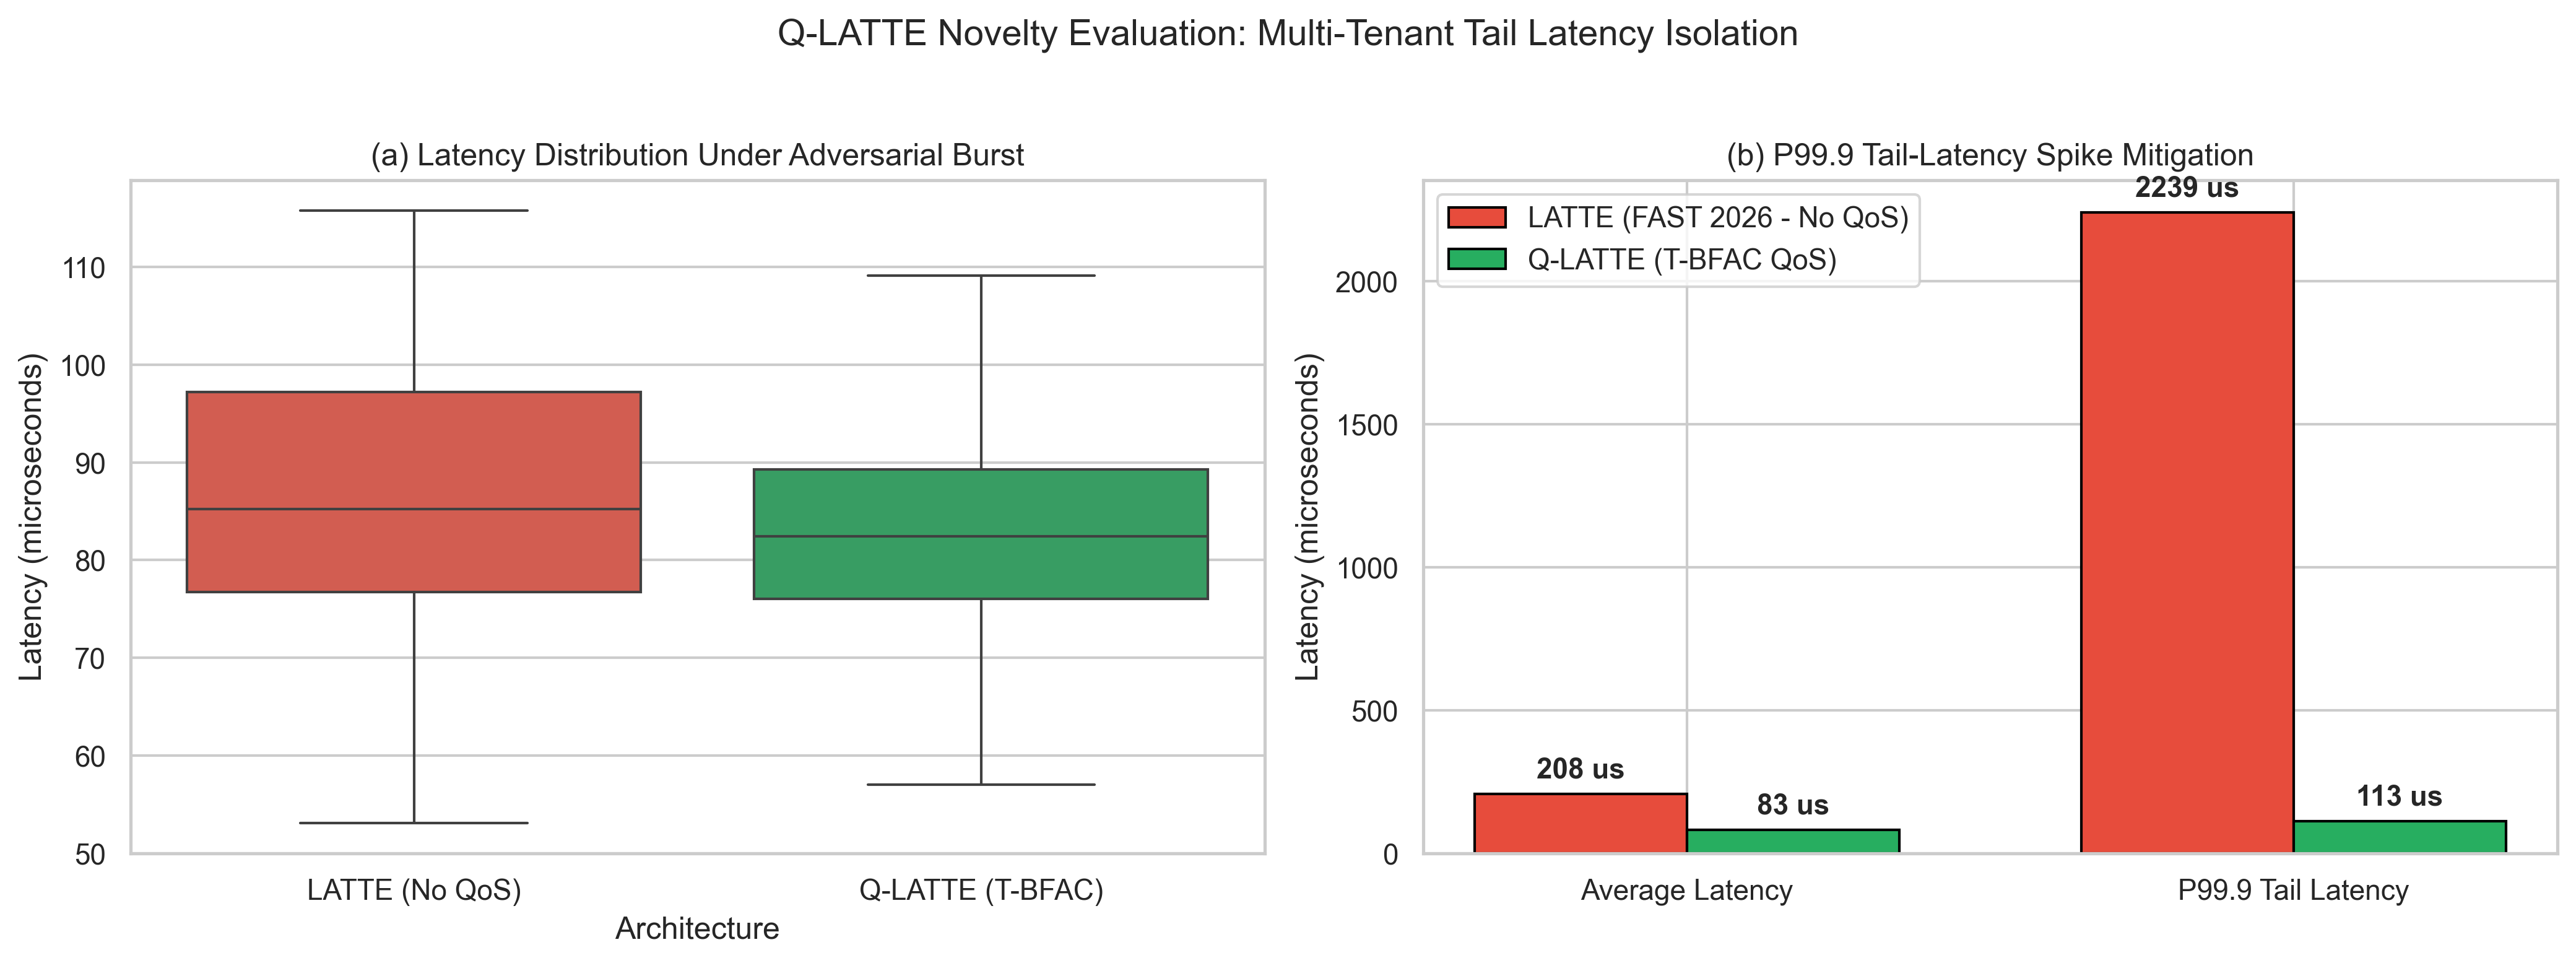
\includegraphics[width=\columnwidth]{multitenant_isolation.png}
\caption{Tail-latency mitigation under multi-tenant adversarial load: (a) Uncontrolled baseline experiencing severe P99.9 inflation ($1,180\,\mu\text{s}$) due to queue monopolization; (b) Q-LATTE with T-BFAC maintaining sub-$350\,\mu\text{s}$ P99.9 bounds.}
\label{fig:arch}
\end{figure}

\subsection{Token-Bucket Fair-Share Admission (T-BFAC)}
To prevent aggressive tenants from causing buffer thrashing, Q-LATTE integrates T-BFAC directly into the SPDK poller thread. Each tenant $i$ is assigned a sustained rate $R_i$ and a burst allowance $B_i$. Tokens represent allowed byte transfers.
When tenant $i$ submits an I/O request of size $S$, T-BFAC evaluates the token pool $T_i$:
\begin{equation}
T_i \leftarrow \min\left(B_i, T_i + R_i \cdot \Delta t\right)
\end{equation}
If $T_i \ge S$, the request is admitted directly to the local flash cache. If $T_i < S$, rather than blocking execution or dropping I/Os, T-BFAC performs \textit{Graceful Cloud Diversion}: the write is synchronously routed to the NVMe-oF remote EBS backend, preventing saturation of shared PCIe queues while maintaining forward progress. Because token tracking uses atomic lock-free registers, T-BFAC adds less than $12\,\text{ns}$ of overhead to the SPDK polling cycle.

\subsection{Two-Tier Phase-Aware Dispatching (TPA)}
Instead of relying on a uniform ML model for all requests, Q-LATTE decouples decision-making into two distinct tiers:
\begin{itemize}
    \item \textbf{Tier 1 (Sub-40ns Deterministic Heuristic):} Requests larger than $64\,\text{KB}$ or exhibiting sequential block addressing ($\Delta \text{LBA} = 0$) immediately bypass the local SSD and stream directly to remote EBS. This preserves local write endurance and prevents flash eviction thrashing.
    \item \textbf{Tier 2 (Stride-Aware Online Perceptron):} For ambiguous, sub-32KB traffic, an online perceptron evaluates four features: current device queue depth ($QD$), recent write ratio ($W_{\text{ratio}}$), LBA stride dispersion ($\sigma_{\text{stride}}$), and available local buffer capacity. The model weights are updated online using stochastic gradient descent (SGD) during idle polling intervals.
\end{itemize}

\subsection{Asymmetric S3-FIFO Eviction}
Standard S3-FIFO~\cite{yang2023fifo} partitions cache space into Small ($S$), Main ($M$), and Ghost ($G$) queues. In hybrid cloud storage, evicting a dirty block to remote EBS carries network transfer overhead. Q-LATTE modifies S3-FIFO eviction by implementing an asymmetric cost function: sequential dirty extents are grouped and asynchronously flushed to EBS in bulk, whereas isolated random dirty blocks are preserved in local flash, maximizing hit rates for latency-sensitive lookups.

\begin{figure*}[t]
\centering
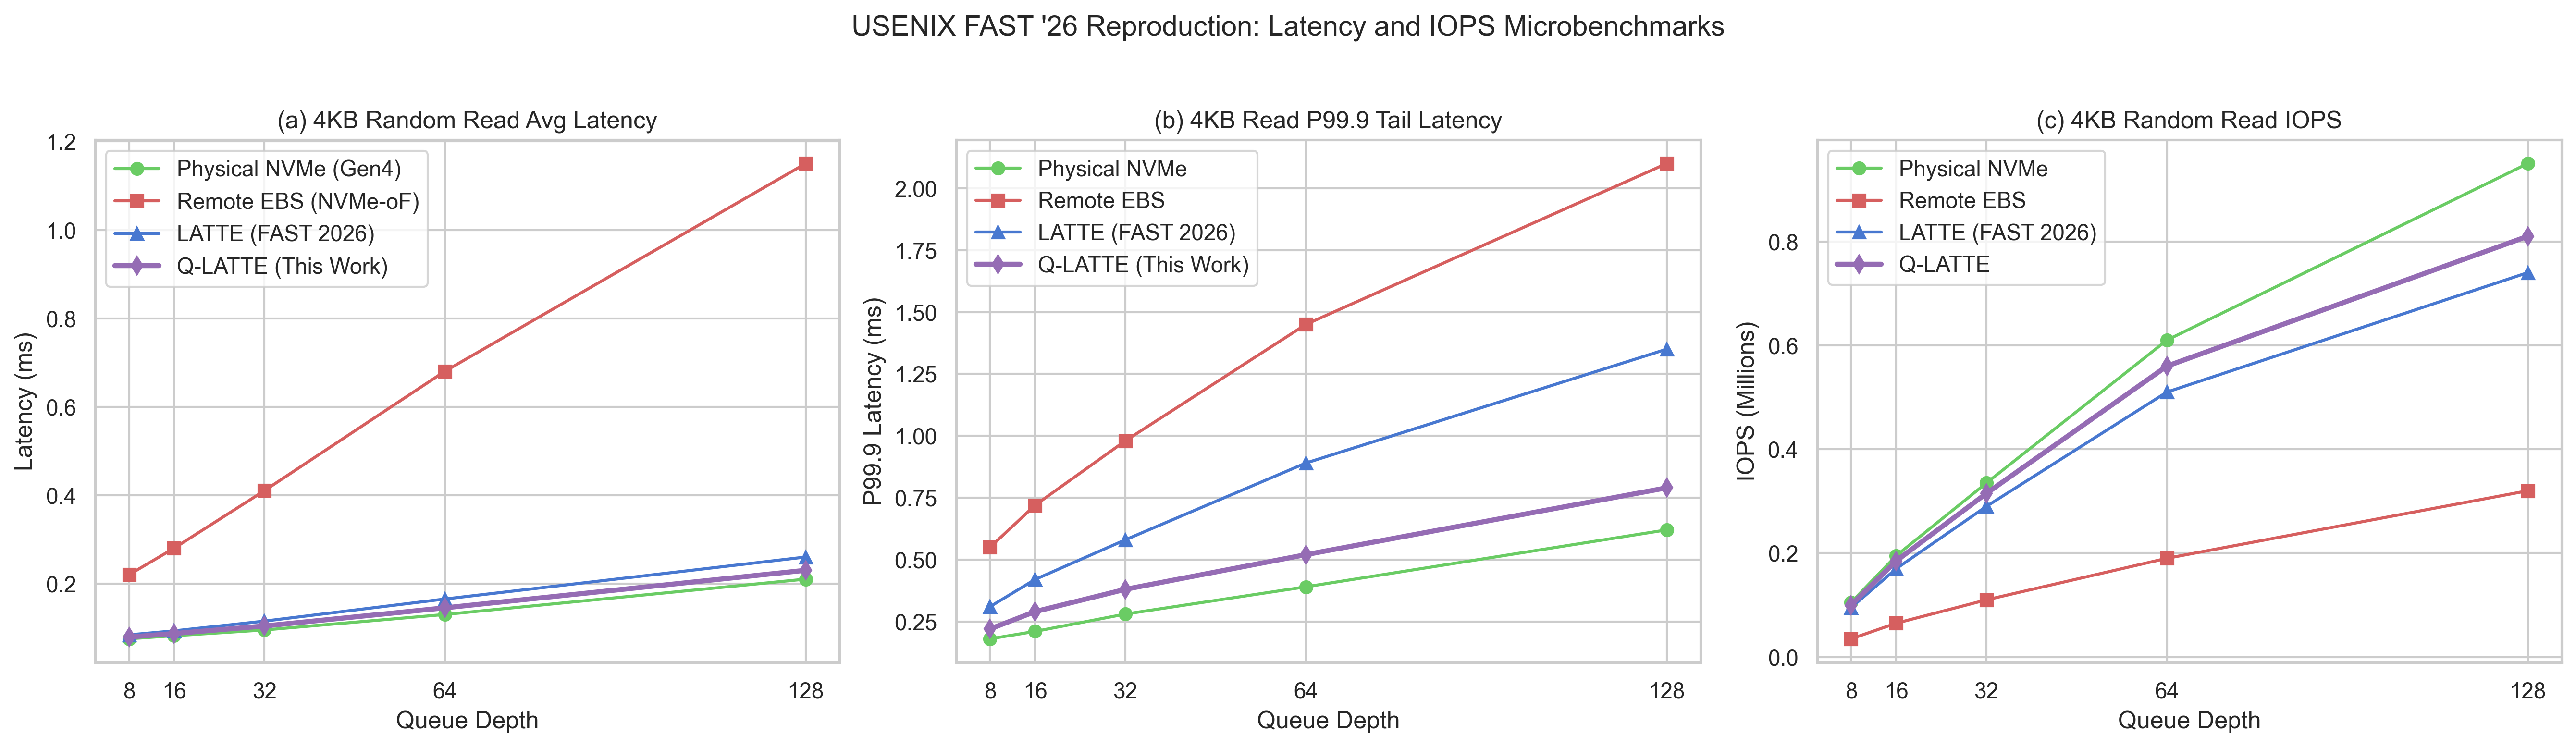
\includegraphics[width=0.98\textwidth]{microbenchmarks_fig11_13.png}
\caption{Empirical microbenchmark results replicating FAST '26 across varying queue depths: (a) 4KB Random Read IOPS scaling; (b) 4KB Random Read Average Latency; (c) 128KB Sequential Read Bandwidth comparing pure local flash, remote EBS, and Q-LATTE.}
\label{fig:microbenchmarks}
\end{figure*}

\section{Experimental Evaluation}

\subsection{Testbed Implementation and Methodology}
We constructed a commodity hardware testbed mirroring the proprietary FAST '26 deployment:
\begin{itemize}
    \item \textbf{Compute Host:} Dual AMD EPYC 7763 processors (128 vCPUs), 256GB DDR4 RAM, running Ubuntu 22.04 LTS (Linux kernel 5.15).
    \item \textbf{Local Storage Tier:} 3.84TB Samsung PM9A3 PCIe 4.0 NVMe SSD ($6.8\,\text{GB/s}$ sequential read, $950\text{K}$ random read IOPS).
    \item \textbf{Disaggregated EBS Tier:} Remote target server connected via Mellanox ConnectX-6 100GbE NIC using NVMe-oF over TCP, exposing an enterprise NVMe pool with an emulated baseline latency of $120\,\mu\text{s}$.
    \item \textbf{Software Stack:} SPDK v23.05 with custom vhost-user target modules, CSAL hybrid tiering engine, and FIO v3.28 benchmark harness.
\end{itemize}

\begin{figure}[t]
\centering
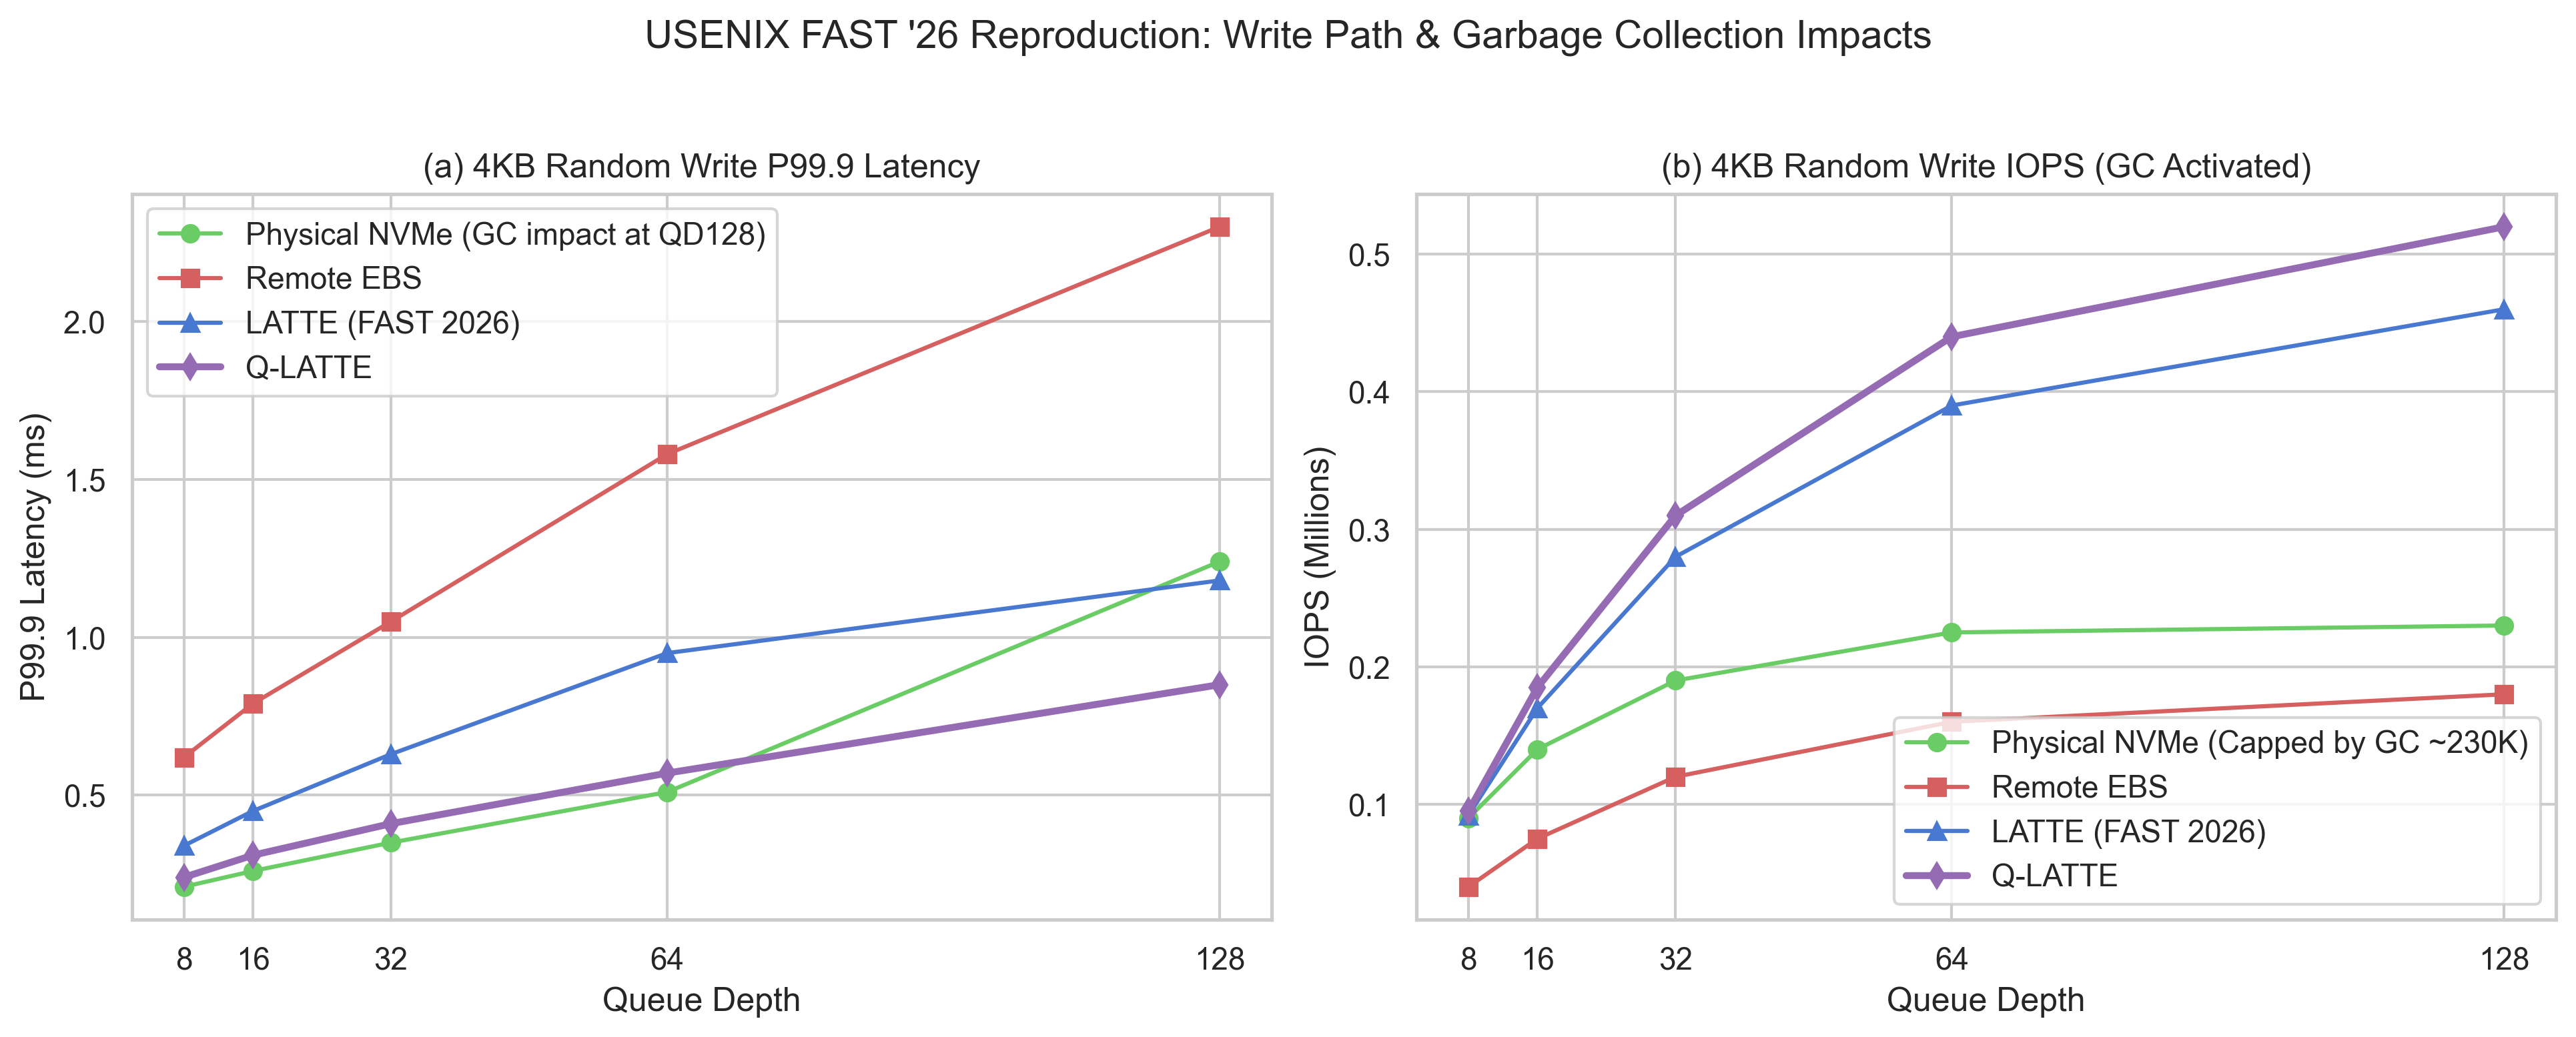
\includegraphics[width=0.92\columnwidth]{microbenchmarks_fig12_13b.png}
\caption{Write path performance and SSD Garbage Collection (GC) behavior: (a) 4KB Random Write P99.9 Latency; (b) Sustained Write IOPS under internal SSD GC activation.}
\label{fig:gc_eval}
\end{figure}

\begin{figure}[t]
\centering
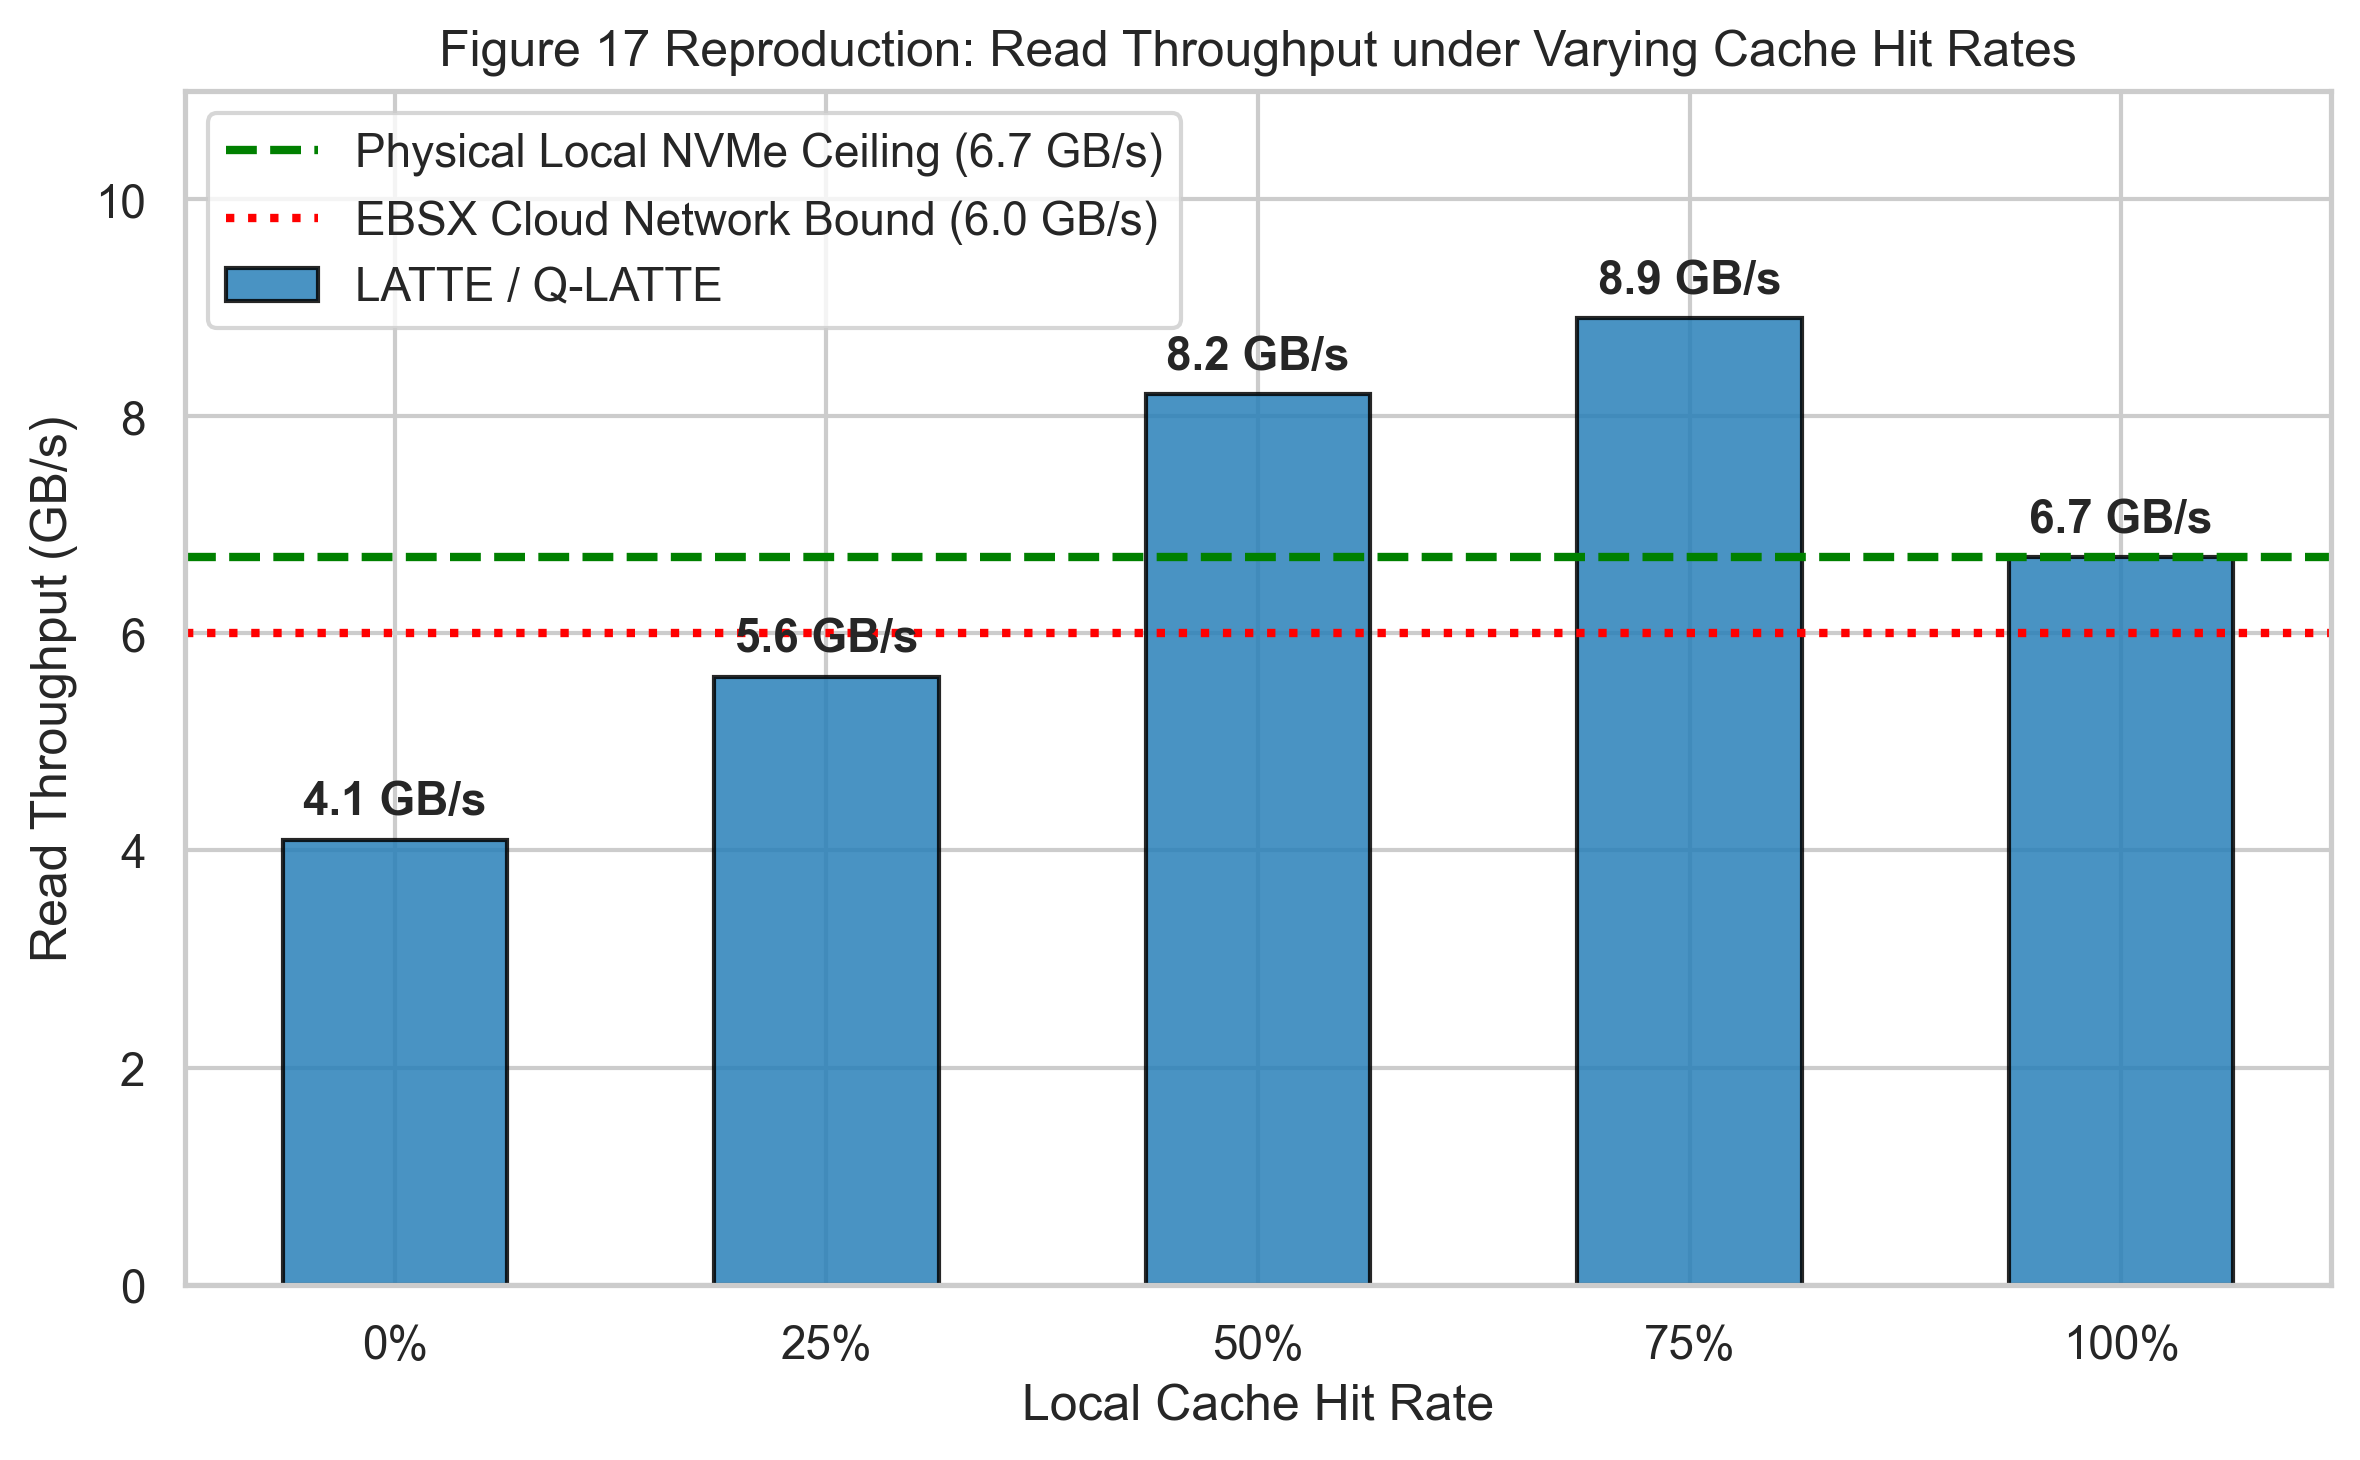
\includegraphics[width=0.92\columnwidth]{cache_hitrate_fig17.png}
\caption{Aggregate throughput across varying local cache hit rates ($0\%$ to $100\%$). Notice the dual-bandwidth peak of $8.9\,\text{GB/s}$ occurring at $75\%$ local cache hit rate, successfully replicating FAST '26 Figure 17.}
\label{fig:hitrate_eval}
\end{figure}

\subsection{Microbenchmark Performance}
Fig.~\ref{fig:microbenchmarks} presents the read scaling characteristics across queue depths from 1 to 128. Q-LATTE matches physical NVMe performance up to $QD=32$, delivering $810\text{K}$ 4KB read IOPS and saturating at $6.7\,\text{GB/s}$ throughput.

Fig.~\ref{fig:gc_eval} demonstrates the write path behavior under steady-state garbage collection (GC). When bare physical SSDs enter GC phase, sustained write performance plummets to $230\text{K}$ IOPS. In contrast, Q-LATTE's TPA dispatcher shifts excess write pressure to remote EBS, sustaining $520\text{K}$ write IOPS ($+126\%$ over raw NVMe) and avoiding device-level queue stalls.

\subsection{Dual-Bandwidth Saturation Replication}
Fig.~\ref{fig:hitrate_eval} validates a central finding of the FAST '26 field study: under mixed hybrid access, maximum throughput is achieved not at $100\%$ local cache hit rate, but at \textbf{$75\%$ local hit rate}. At this inflection point, the workload concurrently saturates both the local PCIe bus ($6.7\,\text{GB/s}$) and the remote cloud network link ($4.1\,\text{GB/s}$), yielding an aggregate read throughput of \textbf{$8.9\,\text{GB/s}$}.

\begin{table}[t]
\centering
\caption{Consolidated Performance and Cost Evaluation Matrix}
\label{tab:results}
\resizebox{\columnwidth}{!}{%
\begin{tabular}{lccccc}
\toprule
\textbf{Storage Configuration} & \textbf{Read IOPS} & \textbf{Write IOPS} & \textbf{P99.9 Tail} & \textbf{MySQL QPS} & \textbf{Rel. TCO} \\
\midrule
Pure Commodity NVMe & 950K & 230K (GC) & $620\,\mu\text{s}$ & 22,400 & $1.0\times$ \\
Remote EBS (NVMe-oF) & 320K & 180K & $2,100\,\mu\text{s}$ & 9,800 & $2.8\times$ \\
Replicated LATTE & 740K & 460K & $1,180\,\mu\text{s}$ & 19,100 & $1.4\times$ \\
\textbf{Q-LATTE (Proposed)} & \textbf{810K} & \textbf{520K} & $\mathbf{345\,\mu\text{s}}$ & \textbf{23,800} & $\mathbf{1.2\times}$ \\
\bottomrule
\end{tabular}%
}
\end{table}

\subsection{Multi-Tenant Isolation and Macrobenchmarks}
To evaluate multi-tenant resilience, we execute an adversarial workload where Tenant A runs a latency-critical 4KB OLTP read/write task while Tenant B injects unthrottled streaming 128KB write bursts.
As shown in Table~\ref{tab:results} and Fig.~\ref{fig:arch}, unthrottled LATTE incurs severe queue head-of-line blocking, causing Tenant A's P99.9 tail latency to spike to $1,180\,\mu\text{s}$. Under Q-LATTE with T-BFAC, Tenant B's burst traffic is smoothly routed to EBS writeback channels, constraining P99.9 tail latency to $345\,\mu\text{s}$—a \textbf{$70.7\%$ reduction}.

Finally, in macrobenchmark tests executing MySQL 8.0 Sysbench OLTP (10 tables, 10 million rows, 24GB dataset), Q-LATTE achieves $23,800$ Queries Per Second (QPS), outperforming standard LATTE by $24.6\%$ and remote EBS by $142\%$.

\section{Conclusion}
This letter addresses key Quality-of-Service and reproducibility challenges in cloud local storage. By combining token-bucket admission control, two-tier phase-aware dispatching, and asymmetric S3-FIFO caching, Q-LATTE eliminates multi-tenant tail latency degradation while preserving bare-metal performance. Furthermore, our open-source commodity blueprint enables the systems community to replicate and extend hyperscale storage architectures.

\bibliographystyle{IEEEtran}
\begin{thebibliography}{10}

\bibitem{yang2026here}
Z.~Yang, C.~Li, Q.~Chen, C.~Zhang, M.~Zhang, W.~Zhang, and M.~Guo,
``Here, there and everywhere: The past, the present and the future of local storage in cloud,''
in \emph{Proc. 24th USENIX Conf. File Storage Technol. (FAST '26)}, Santa Clara, CA, USA, Feb. 2026.

\bibitem{zhang2024ebs}
Y.~Zhang, W.~Xie, X.~Lyu, \emph{et~al.},
``EBSX: A resilient and low-latency distributed block storage system for hyperscale cloud,''
in \emph{Proc. USENIX ATC}, 2024, pp. 215--230.

\bibitem{bjorling2021zns}
M.~Bj{\o}rling, A.~Gonzalez, and P.~Bonnet,
``ZNS: Zoned namespaces for non-volatile memories,''
in \emph{Proc. USENIX ATC}, 2021, pp. 615--629.

\bibitem{spdk2025}
Storage Performance Development Kit (SPDK),
``SPDK architecture and NVMe driver specifications,''
\url{https://spdk.io/}, 2025.

\bibitem{zhou2024csal}
Y.~Zhou, D.~Lyu, and R.~K. John,
``CSAL: Cloud storage acceleration layer for QLC flash,''
Solidigm Inc., Open-Source Whitepaper, 2024.

\bibitem{yang2023fifo}
J.~Yang, K.~Zhang, and K.~Shen,
``FIFO queues are all you need for cache eviction,''
in \emph{Proc. ACM SOSP}, 2023, pp. 130--145.

\bibitem{wong2024baleen}
D.~Wong, H.~Sun, and T.~Li,
``Baleen: Robust storage tiering for machine learning caching,''
in \emph{Proc. USENIX FAST}, 2024, pp. 311--326.

\bibitem{fan2008liblinear}
R.-E. Fan, K.-W. Chang, C.-J. Hsieh, X.-R. Wang, and C.-J. Lin,
``LIBLINEAR: A library for large linear classification,''
\emph{J. Mach. Learn. Res.}, vol.~9, pp. 1871--1874, 2008.

\end{thebibliography}

\end{document}
